
\documentclass[a4paper,10pt]{article}

\usepackage[utf8x]{inputenc}
\usepackage[textwidth=160mm,textheight=229mm]{geometry}
\usepackage{graphicx}
\usepackage{amsmath}
\usepackage{fancybox}
\usepackage{cancel}
\usepackage{wrapfig}
\usepackage{amsmath,amssymb,amsfonts,mathrsfs}
\usepackage{color}
\usepackage{slashed}
\usepackage{bbm}
\usepackage{xspace}
\usepackage{subcaption}
\usepackage{multicol}
\usepackage{tikz}
\usepackage{hyperref}


\title{\textbf{Opportunities at MeLi Code Excercise Data Scientist}}

\author{Felipe Rojas Abatte}

\begin{document}
\maketitle
%\tableofcontents

\section*{Introducci\'on}
En el contexto del Marketplace de MercadoLibre se necesita un algoritmo para predecir si un artículo listado en el mercado es \textbf{nuevo} o \textbf{usado.}
Sus tareas implican el an\'alisis de datos, el dise\~no, el procesamiento y el modelado de una solución de aprendizaje automático para predecir si un artículo es nuevo o usado y luego evaluar el modelo a partir de datos de prueba disponibles.
Para ayudar en esa tarea, se proporciona un conjunto de datos en \textbf{MLA\_100k\_checked\_v3.jsonlines} y una función \textbf{build\_dataset} para leer ese conjunto de datos en \textbf{new\_or\_used.py}.
Para la evaluación, utilizará la métrica de precisión para obtener un resultado de 0,86 como mínimo. Además, deberá elegir una métrica secundaria adecuada y también elaborar un argumento sobre por qué se eligió esa métrica.

\section*{Entregables}

\begin{itemize}
\item El archivo, incluido todo el código necesario para definir y evaluar un modelo.
\item Un documento con una explicación sobre los criterios aplicados para elegir las características, la métrica secundaria propuesta y el rendimiento alcanzado en esas métricas. 
\item Opcionalmente, puede entregar un análisis EDA con otro formato como .ipynb
\end{itemize}

\newpage

\section*{Selección de features}
El análisis del conjunto de datos provenientes del archivo \textbf{MLA\_100k\_checked\_v3.jsonlines} originalmente contenidos en formato json, por lo cual, fue necesario realizar un 
preprocesamiento de datos considerando la transformación del archivo json en un dataframe, posterior \textbf{aplanamiento} de algunas columnas anidadas (non\_mercado\_pago\_payment\_methods,
pictures) y finalizando con la limpieza de carácteres especiales como contenidas en otras columnas (sub\_status, deal\_ids, variations, attributes, tags, coverage\_areas, descriptions,
shipping.methods, shipping.tags). Este proceso fue realizado a través de la función \texttt{clean\_flattern\_json} del código python.
\newline
Una vez realizado este proceso se lograron reconocer 3 tipos de datos: datos numéricos, categóricos y booleanos.
El primer filtro o criterio de eliminación de columnas del dataframe fue considerar aquellas que:
\begin{itemize}
    \item tuvieran datos faltantes,
    \item tuvieran valores nulos o NaN
    \item tuvieran espacios en blanco
    \item tuvieran el mismo dato replicado en todas las filas (0 \% de  variabilidad)
    \item tuvieran en cada fila un dato distinto (100 \% de variabilidad)
\end{itemize}

El segundo criterio de eliminación de columnas del dataframe fue considerar aquellas que aportaban exactamente la misma información, por ejemplo:
\begin{itemize}
    \item seller\_address.country.name contiene la misma información que seller\_address.country.id
    \item seller\_address.state.id contiene la misma informacion que seller\_address.state.name
    \item seller\_address.city.id contiene la misma informacion que seller\_address.city.name
    \item non\_mercado\_pago\_payment\_methods.id contiene la misma informacion que .description
\end{itemize}

El tercer criterio de eliminación fue considerar la importancia de las variables utilizando a través del uso de un algoritmo de tipo random forest.
Los resultados obtenidos muestran que las variables asociadas a fecha: dia, semana, mes y año además de diff\_time son las que menos aportan al modelo, por lo tanto no las consideraremos en el entrenamiento.
\begin{figure}[htb]
\centering
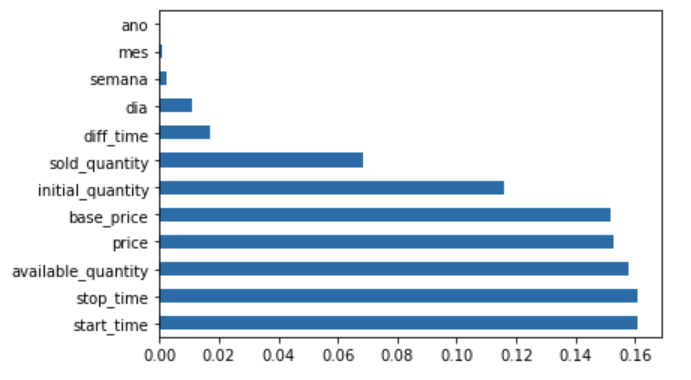
\includegraphics[width=0.6\textwidth]{./pictures/importance.png}
\caption{Importancia entre variables continuas} \label{import}
\end{figure}  
\newline  
El cuarto criterio de eliminación fue realizar un análisis de correlación sobre las variables continuas para identificar aquellas que presentan mayor independencia,
y de esa manera reducir el riesgo de multicolinealidad.
\begin{figure}[htb]
\centering
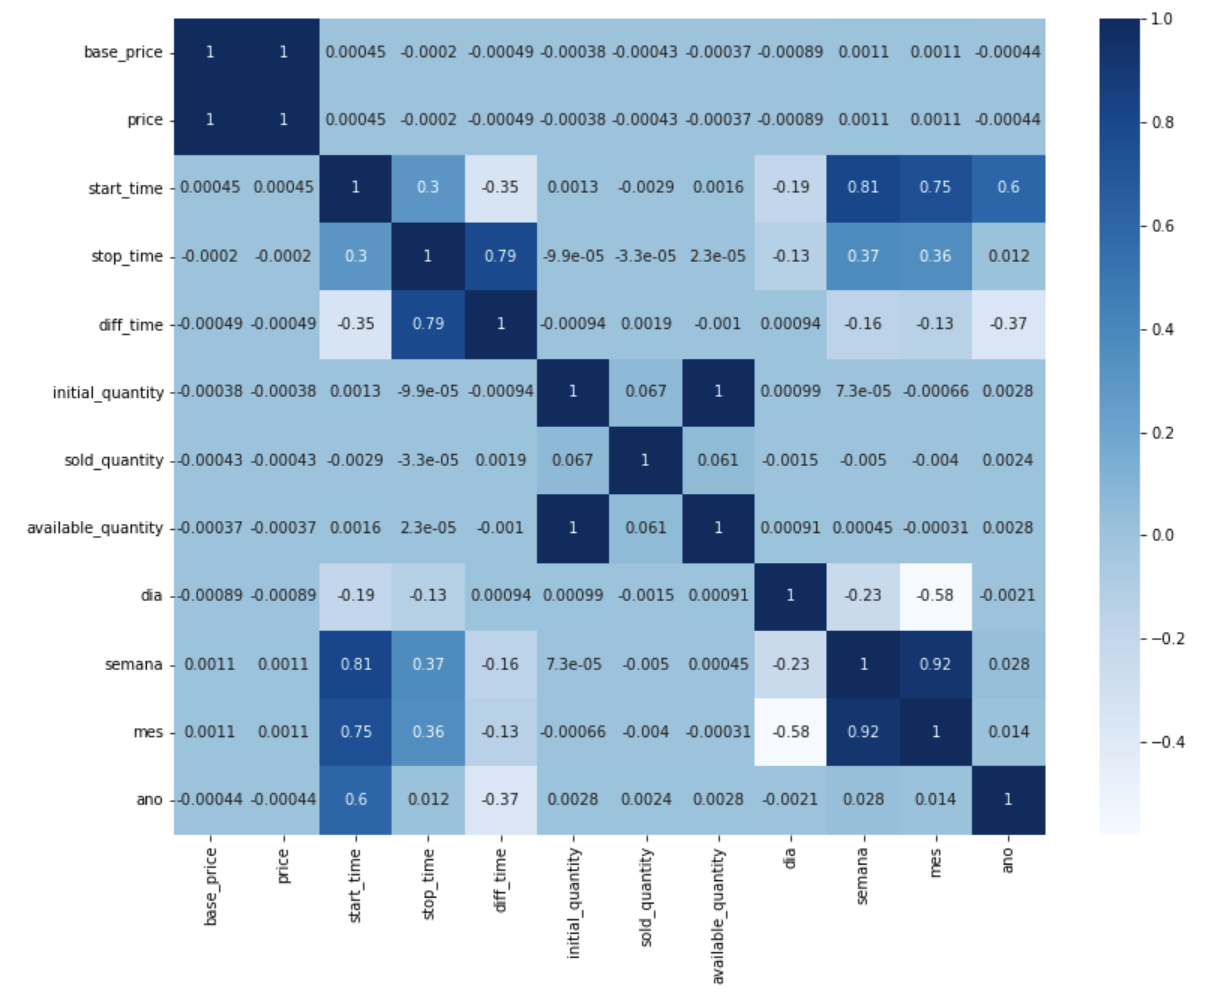
\includegraphics[width=0.6\textwidth]{./pictures/corr.png}
\caption{Correlación entre variables continuas} \label{corr}
\end{figure}    
El resultado muestra que las variables \textit{base\_price} y \textit{price} presentan un alto grado de correlación. De la misma forma las variables \textit{initial\_quality}
y \textit{available\_quality} también presentan un alto grado de correlación.
\newline
Finalmente no consideraremos toda la sección de variables \textit{pictures} dado a que contienen información con mucha variabilidad. De esta menera las variables a considerar 
para el entrenamiento del modelo son: \newline
\textbf{Numerical features}
\begin{itemize}
    \item stop\_time
    \item start\_time
    \item available\_quantity
    \item price
    \item initial\_quantity
    \item sold\_quantity
\end{itemize}
\textbf{Categorical features}
\begin{itemize}
    \item buying\_mode
    \item accepts\_mercadopago
    \item currency\_id
    \item automatic\_relist
    \item status
    \item seller\_address.state.name
    \item seller\_address.city.name
    \item shipping.local\_pick\_up
    \item shipping.free\_shipping
    \item shipping.mode
    \item non\_mercado\_pago\_payment\_methods.description
    \item no\_mercado\_pago\_payment\_methods.type
\end{itemize}
                       
\section*{Segunda métrica de desempeño}
La segunda métrica de evaluación para el desempeño del modelo que utilizaré será \textbf{classification\_report}. 
Esta métrica muestra un resumen completo del desempeño de un clasificador utilizando en su conjunto varias métricas de evaluación. 
Ayuda a evaluar la capacidad del modelo para clasificar correctamente diferentes clases, proporcionando información sobre el rendimiento de cada clase y la calidad general del modelo.
La métrica de \textbf{classification\_report} tiene varias ventajas por sobre la \textbf{Accuracy}:
\begin{itemize}
\item Proporciona una evaluación más detallada del rendimiento del modelo. Considera dentro del reporte métricas como precisión, recall y F1-score para cada clase, 
      lo que brinda más información sobre el rendimiento del modelo en clases individuales. La Accuracy, por otro lado, solo proporciona un valor único que 
      representa el rendimiento general del modelo.
\item Manejo de datos desequilibrado. Cuando se trabaja con conjuntos de datos desequilibrados, donde algunas clases tienen menos datos
      que otras, la Accuracy puede ser engañosa. Un modelo puede funcionar bien en la clase mayoritaria pero mal en las clases minoritarias y aun así tener una 
      alta precisión. El informe de clasificación proporciona métricas para cada clase, lo que facilita la identificación y solución de este problema.
\item Equilibra la precisión y recall: la puntuación F1 en el informe de clasificación proporciona un equilibrio entre precisión y recall, dando igual 
      importancia a los falsos positivos y los falsos negativos. Esto es particularmente importante en situaciones donde ambos tipos de errores tienen consecuencias 
      similares. 
\item Identifica áreas de mejora. El informe de clasificación ayuda a identificar clases en las que el rendimiento del modelo es deficiente, proporcionando 
      información sobre posibles áreas de mejora. Al centrarse en las métricas de cada clase, se pueden comprender mejor las debilidades del 
      modelo y realizar los ajustes necesarios.
\end{itemize}
Al aplicar Ambas métricas de evaluación del desempeño del modelo Random Forest los resultados se muestran a continuación
\begin{figure}[htb]
    \centering
    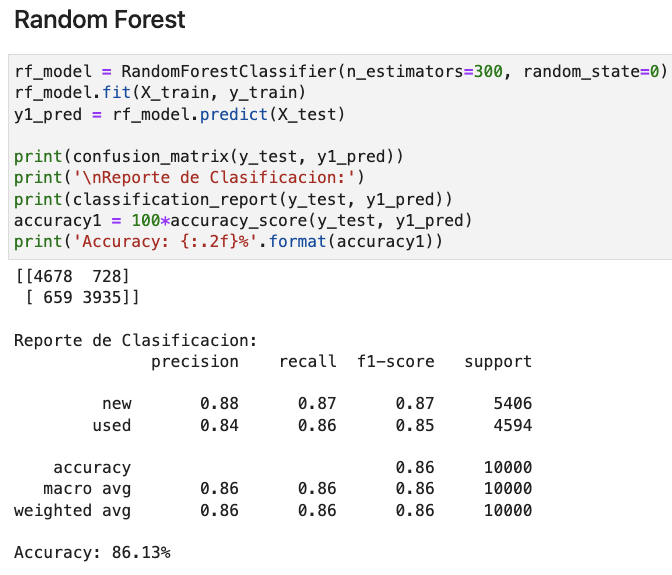
\includegraphics[width=0.6\textwidth]{./pictures/model_result.png}
    \caption{Metricas de desempeño del modelo seleccionado (Random Forest)} \label{best_model}
    \end{figure}  
\end{document}